\documentclass[runningheads]{llncs}

%---- Sonderzeichen-------%
\usepackage[english]{babel}
%---- Codierung----%
\usepackage[latin1]{inputenc}	% for Unix and Windows
\usepackage[T1]{fontenc}
\usepackage{graphicx}
\usepackage{url}
\usepackage{llncsdoc}
%----- Mathematischer Zeichenvorrat---%
\usepackage{amsmath}
\usepackage{amssymb}
\usepackage{enumerate}
% fuer die aktuelle Zeit
\usepackage{scrtime}
\usepackage{listings}
\usepackage{subfigure}
\usepackage{hyperref}
\usepackage{float}

\setcounter{tocdepth}{3}
\setcounter{secnumdepth}{3}

%https://github.com/cocome-community-case-study/cocome-cloud-jee-platform-migration/blob/master/cocome-maven-project/doc/Deployment%20Setup.md

\begin{document}
\title{Docker Evolution Scenario}
\author{Benkler, Niko; Ha�berg, Tobias; Heinrich, Robert}
\institute{Institute for Program Structures and Data Organization}
\maketitle
\section{Docker}\label{docker}
Docker is an open source software using container technology to isolate applications on a system. \\
	An advantage of using this technology is the higher efficiency in the consumption of hardware resources by running independent containers on a single Linux Kernel and avoiding the overhead of maintaining virtual machines. Therefore, this technology provides higher efficiency compared to similar solutions using virtual machines.
	Independent containers run on a single Linux Kernel avoiding the overhead of maintaining virtual machines. Therefore, this technology provides higher efficiency compared to VMs, as it does not consume as much hardware resources. Furthermore, there is no need to manually install software that is necessary to run the application, as the Dockerfile specifies the environment in which the application is able to run. \\
	Docker builds a so-called \textit{Image} by using a Dockerfile. Starting from an empty server environment, Docker executes the commands of the Dockerfile to set up the docker container, the application environment and the application itself.\\
	Docker can be forced to download the newest  software version, if available, when building a new Image. This is usually done in the Dockerfile specification. As a consequence, the application itself and the software it uses will always be up to date.\\
	The docker environment is suitable for efficiently running various containers at a time. It is therefore predestined for Microservice-based applications, as the different Services can be deployed independently in a container. 

\section{Docker for CoCoME}
	As described in the CoCoME installation guide, CoCoME needs a bunch of software that has to be installed manually. This platform dependant software needs to be kept up to date, no matter on what kind of system it will be deployed. The basic idea behind \textit{Docker for CoCoME} is to create a platform independent version which does not require any manual installation by a person apart from Docker itself. 
	

\section{Evolution Scenario}
	Within several steps, CoCoME became more complex. This includes further software that has to be installed to run CoCoME.\\ 
	The main objective in this evolution scenario is to provide a platform independent version of CoCoME that does not require any preconditions like installing or updating  software. In this case, Docker is a suitable alternative.\\
	By using Docker, CoCoME can be instantiated on any device without installing additional software.
	
\section{Implementation Overview}
	Implementing the \textit{Dockerfile} turned out to be the main part of this evolution scenario. It defines the way in which the technology stack is extended. The installation is described in detail in section \ref*{description}.\\ 
	Briefly, we are using a Docker container that provides a full Linux distribution and deploys all needed software to accomplish the installation of CoCoME as described in the official  CoCoME installation guide\footnote{\url{https://github.com/cocome-community-case-study/cocome-cloud-jee-platform-migration/blob/master/cocome-maven-project/doc/Deployment\%20Setup.md}}.


\section{Description}\label{description}
	As shown in figure \ref*{techStack} the changes are affecting the technology stack by adding additional layers. More detailed, the given CoCoME Stack is moved into the Docker Deamon, which runs a Linux distribution.As mentioned before, Glassfish and the JVM are still part of the CoCoME Stack.
	\\
\begin{figure}[H]
	\centering
	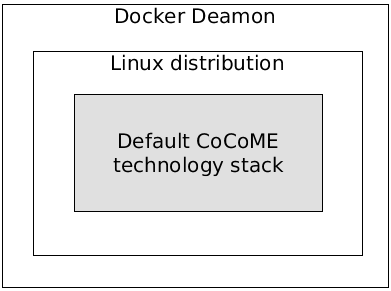
\includegraphics[width = 0.5\textwidth]{img/tech_stack_CoCoME.png}
	\caption{Extended technology stack CoCoME}
	\label{techStack}
\end{figure}

	The Dockerfile defines an environment based on the latest version of Ubuntu 16:04. Maven, Git and Java are installed on top of Ubuntu using Ubuntu's default package manager.\\
	Git has two purposes: On the one hand it is used to download the most recent version of CoCoME. On the other hand, it is used to download a prefabricated version of Glassfish that already includes domains and other adjustments required for CoCoME. Java is required by Glassfish and CoCoME as they need the Java Virtual Machine. Maven is needed to deploy the latest version of CoCoME onto the provided Glassfish servers.

\section{Deployment}
	During the development, it was decided to implement and to provide two different versions. The first version always pulls the most recent CoCoME source code from GitHub, downloads the entire dependencies with Maven, compiles and builds the project and finally, deploys CoCoME on the Glassfish servers. As a consequence. creating and starting a Docker Container takes about one hour.
	In contrast, the second version only  pulls a prefabricated version of CoCoME from GitHub. Therefore, pulling the source code up to building the project is skipped. As a consequence, Maven does not have to be included in the technology stack. Solely, deploying CoCoME on the Glassfish server is necessary.\\
	This reduces the deployment time to a few minutes but has a disadvantage: The prefabricated version is updated manually. Therefore, it is sometime not the most recent version.
	By providing both, a fast deploying version and a current version, the user can choose what's the best for its situation.
	
\begin{figure}[h]
	\centering
	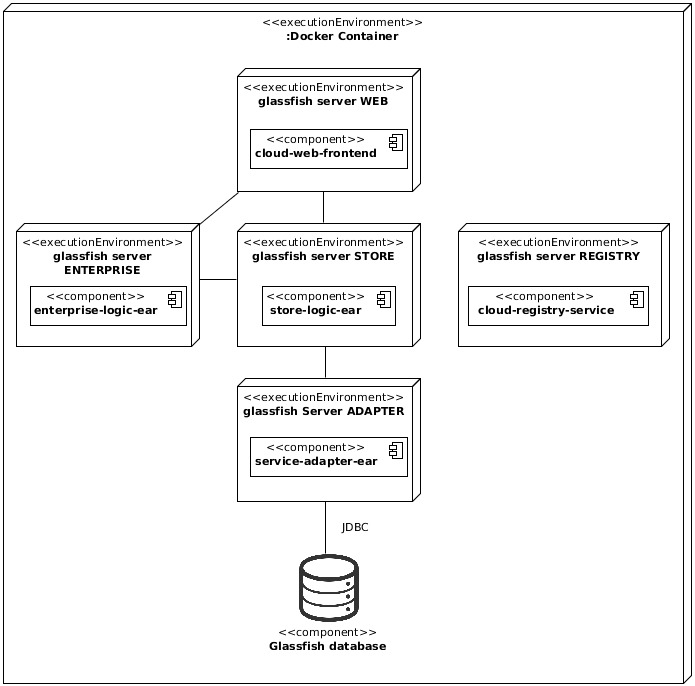
\includegraphics[width = 0.9
	\textwidth]{img/docker_Container_Deployment.png}
	\caption{Deployment diagram CoCoME}
	\label{Deploym_CoCoME}
\end{figure}

	As shown in Fig. \ref*{Deploym_CoCoME} the docker Container contains five different Glassfish servers. In particular they are called \textit{WEB}, \textit{ENTERPRISE}, \textit{STORE}, \textit{REGISTRY} and \textit{ADAPTER} and correspond to the recommendations given by the CoCoME deployment setup. By default, Glassfish provides a Derby DB that is connected to the server Adapter using Java Database Connectivity (JDBS) interface.\\
	As mentioned before, CoCoME is deployed inside the docker container on the same way it is usually deployed. This means the Maven generated archive files \textit{cloud-web-frontend},\textit{enterprise-logic-ear},\textit{store-logic-ear}\textit{cloud-registry-sevice} and \textit{service-adapter-ear} are deployed to the servers with the following assignment:
	
	\begin{figure}[H]
		\centering
		\begin{tabular}{p{0.25\textwidth}|p{0.01\textwidth}p{0.25\textwidth}}
			Server && Deployment file \\
			\hline
			WEB && cloud-web-frontend  \\
			ENTERPRISE && enterprise-logic-ear  \\
			STORE && store-logic-ear  \\
			REGISTRY && cloud-registry-service  \\
			ADAPTER && service-adapter-ear \\	
		\end{tabular}
		\caption{Assignment of archive files to Servers}
		\label{table_assignment}
	\end{figure}
	Fig. \ref{table_assignment} demonstrates the assignment between the archive files and the servers as it is implemented and also recommended by the CoCoME deployment guide. This information is also represented in Fig. \ref{Deploym_CoCoME}. The two different Docker versions both use this assignment.
	In addition, the fast version can be extended by the Pickup Shop\footnote{\url{https://github.com/cocome-community-case-study/cocome-cloud-jee-web-shop}}. This extension runs inside a separate container which is shown in Fig. \ref{Deploym_Pickup}. It basically uses the same technology stack.	As shown in Fig. \ref*{Deploym_Pickup}, this container provides only one Glassfish server.
	\begin{figure}[H]
		\centering
		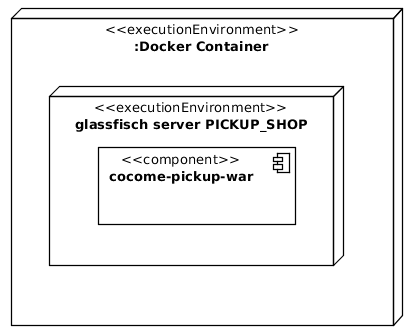
\includegraphics[width = 0.4\textwidth]{img/docker_Container_PickUP.png}
		\caption{Deployment diagram CoCoME Pickup Shop}
		\label{Deploym_Pickup}
	\end{figure}

	\begin{figure}[H]
		\centering
		\begin{tabular}{p{0.25\textwidth}|p{0.01\textwidth}p{0.25\textwidth}}
			Server && Deployment file \\
			\hline
			PICKUP\_SHOP && cocome-pickup-war \\	
		\end{tabular}
		\caption{Assignment archive files to Servers}
		\label{table_assignment_pickup}
	\end{figure}

	To control the start of both containers, precisely the CoCoME and the Pickup Shop, another specific file is needed: the Docker Compose file. It ensures that the CoCoME Container is active before the Pickup Shop container starts. This is necessary as the Pickup Shop requires a running instance of CoCoME to register itself.\\
	Whereas CoCoME does not require the Pickup Shop, the inversion is not correct. \\
	Both containers need to communicate with each other. By default, docker prohibits any outgoing and ingoing communication from an in a container. This is solved by opening specific ports through which the communication is possible. Which ports the containers can use is specified in the Docker Compose file as well.
\end{document}
